\section{Theorie}
\label{sec:Theorie}

\subsection{Fehlerrechnung}

Für die Fehlerfortpflanzung bei Gleichungen mit $N$ fehlerbehafteten Größen
wird jeweils die Formel zur Gaußschen Fehlerfortpflanzung

\begin{equation}
  \sigma = \sqrt{\sum_{i=1}^{N}\biggl(\frac{\partial f(x_i)}{\partial x_i}
  \sigma_i\biggr)^2}
\end{equation}
mit der jeweiligen Funktion $f(x_i)$, den Messgrößen $x_i$ und den
zugehörigen Fehlern $\sigma_i$ verwendet.
Zur Berechnung des arithmetischen Mittels von $N$ Messwerten wird jeweils die
Formel

\begin{equation}
  \bar{x} = \frac{1}{N}\sum_{i=1}^{N}x_i
\end{equation}
mit den Messwerten $x_i$ benutzt.
die Standardabweichung des Mittelwerts wird jeweils mit der Gleichung

\begin{equation}
  \bar{\sigma} = \sqrt{\frac{1}{N-1}\sum_{i=1}^{N}(x_i - \bar{x})^2}
\end{equation}
mit den $N$ Messwerten $x_i$ berechnet.

\subsection{Einleitung und Zielsetzung}

Im folgenden Versuch sollen die Spektren der Alkali-Metalle im sichtbaren
Bereich des elektromagnetischen Spektrums untersucht werden. Aus den
Energien der angeregten Zustände eines Atoms kann die Stärke des
Coulombfelds an dem jeweiligen Ort des betrachteten Elektrons im Atom
bestimmt werden. Dabei ist
zu beachten, dass die Elektronen auf inneren Schalen das Coulombfeld abschwächen.
Man führt die Abschirmkonstante $\sigma$ ein und für die
effektive Kernladung gilt
\begin{align}
  z_\text{eff} = z - \sigma.
\end{align}
Die Alkali-Metalle haben alle die Eigenschaft, dass sie jeweils ein
Leuchtelektron besitzen. Das bedeutet, dass
die Atome jeweils aus einem Atomrumpf, das ist der Atomkern mit allen
abgeschlossenen Schalen, und einem äußeren Elektron bestehen. Diese
Eigenschaft wird bei einigen der folgenden Rechnungen mit Hilfe der sogenannten
Ein-Elektonen-Näherung ausgenutzt. An dieser Stelle lässt sich
bereits vermuten, dass eine Ähnlichkeit zwischen den Alkali-Spektren und dem
Wasserstoff-Spektrum besteht, da Wasserstoff ebenfalls in der Hauptgruppe der
Elemente mit nur einem Valenz-Elektron ist.

\subsection{Einführung der Quantenzahlen und relativistische Effekte}

Zunächst wird die stationäre Schrödingergleichung für die Teilchen im Atom
aufgestellt
\begin{align}
  H \psi = E \psi.
  \label{eqn:statSchroed}
\end{align}
Dabei ist
\begin{align}
  H = \frac{P^2}{2 m_0} - U(r)
\end{align}
der Hamitonoperator, wobei
\begin{align}
  U(r) = - \frac{(z-\sigma) e_0^2}{4 \pi \epsilon_0 r}
\end{align}
das genäherte Potential des Kernfelds und
\begin{align}
  P = \frac{\hbar}{i} \nabla
\end{align}
der Impuls ist.
Da es sich um ein radialsymmetrisches Problem handelt, werden Kugelkoordinaten
und damit die sogenannte Bahndrehimpulsquantenzahl $l$ eingeführt. Für diese
Quantenzahl gilt stets die Beziehung
\begin{align}
  l_\text{max} = n-1
\end{align}
mit der Hauptquantenzahl $n$.
Beachtet man relativistische Effekte, so muss der Hamiltonoperator zu
\begin{align}
  H_\text{rel} = \sqrt{m_0^2 c^4 + c^2 P^2} - m_0 c^2 + U
\end{align}
umgeformt werden. In einer Näherung werden diese Effekte als Störungen
behandelt und nach einer aufwendigen Rechnung ergibt sich die für die
Schrödingergleichung \eqref{eqn:statSchroed} gesuchte Energie in Abhängigkeit
von den Quantenzahlen $n$ und $l$
\begin{align}
  E_{n,l} = -R_\infty \biggl(\frac{(z-\sigma)^2}{n^2} + \alpha^2 \frac{(z-\sigma)^4}{n^3}
  \Bigl(\frac{2}{2l+1} - \frac{3}{4n}\Bigr) \biggr).
\end{align}
Dabei ist
\begin{align}
  \alpha = \frac{e_0^2}{2 h c \epsilon_0}
\end{align}
die Sommerfeldsche Feinstrukturkonstante und
\begin{align}
  R_\infty = \SI{13.6}{\electronvolt}
\end{align}
die Rydberg-energie.
Berücksichtigt man die Tatsache, dass die Elektronen frei sind und somit einen
Spin haben, so muss zusätzlich die Spinquantenzahl $j$
eingeführt werden. Da Bahndrehimpuls und Spin nur parallel oder antiparallel
zueinander sein können, folgen sofort die Beziehungen
\begin{align}
  j = l \pm \frac{1}{2}.
  \label{eqn:SpinBahn}
\end{align}
Zwischen den verschiedenen, aus den Drehimpulsen entstehenden, magnetischen
Momenten der Elektronen entstehen nicht vernachlässigbare Wechselwirkungen, die
auch als Spin-Bahn-Kopplung bezeichnet werden.
Diese Effekte können genähert werden, sodass sich für die Energieeigenwerte
in Abhängigkeit von $n$ und $j$
\begin{align}
  E_{n,j} = -R_\infty \biggl(\frac{(z-\sigma)^2}{n^2} + \alpha^2 \frac{(z-\sigma)^4}{n^3}
  \Bigl(\frac{1}{j+\frac{1}{2}} - \frac{3}{4n}\Bigr)\biggr)
  \label{eqn:SommerFormel}
\end{align}
ergibt, wobei $l$ bereits mit der Beziehung \eqref{eqn:SpinBahn} durch $j$
ausgedrückt wird.
Diese Gleichung \eqref{eqn:SommerFormel} entspricht in erster Näherung der
Sommerfeldschen Feinstrukturformel.
Zur Kurzschreibweise der Energieniveaus werden die Quantenzahlen durch zwei
Zahlen und einen Buchstaben geschrieben.
Für die Bahndrehimpulsquantenzahl $l$ wird ein Großbuchstabe wie folgt
geschrieben:
\begin{align}
  l = & 0 & \text{"S"} \\
  l = & 1 & \text{"P"} \\
  l = & 2 & \text{"D"} \\
  l = & 3 & \text{"F"}.
\end{align}
Die Hauptquantenzahl $n$ wird vor den Buchstaben geschrieben und die
Spinquantenzahl $j$ als Index dahinter.

\subsection{Energieniveauübergänge und Auswahlregeln}

Die Elektronen um einen Atomkern können durch äußere Anregung ihr eigenes
Energieniveau ändern und beispielsweise auf eine niedrigere Schale springen.
Bei solchen Energieübergängen ändern sich die Quantenzahlen und es wird
Energie in Form von Strahlung abgegeben. Allerdings sind nicht alle möglichen
Energieübergänge im Atom erlaubt. Solche mit
\begin{align}
  \increment j = 0
\end{align}
sind sehr unwahrscheinlich und für $l$ sind nur Übergänge mit
\begin{align}
  \increment l = \pm 1
\end{align}
erlaubt. Bei der Hauptquantenzahl werden die Sprünge mit steigendem
$\increment n$ unwahrscheinlicher.
Die Energieniveaus mit gleichem $l$ und unterschiedlichem $j$ liegen
deutlich näher aneinander als diejenigen mit unterschiedlichem $l$, weshalb
im Spektrum Dubletts erkennbar sind. In Abbildung \ref{fig:enueber} wird dieses
Phänomen dargestellt.

\begin{figure}
  \centering
  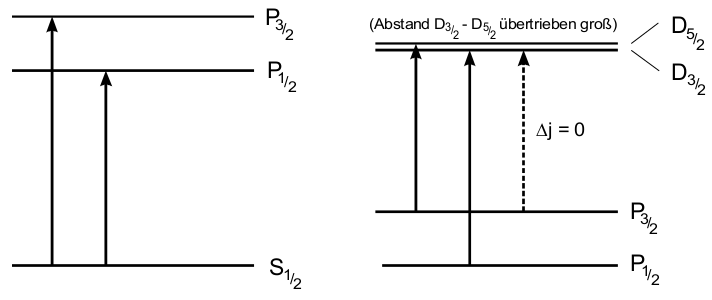
\includegraphics[height=5cm]{MeinFotoalbum:)/Energieuebergaenge.png}
  \caption{Skizze zur Lage der Spektrallinien in einer Dublettstruktur.
  \cite{anleitung}}
  \label{fig:enueber}
\end{figure}

\subsection{Abschirmungskonstanten}

Bei den Abschirmungszahlen, die zur Berechnung der Eigenenergien bestimmt
werden müssen, unterscheidet man zwischen der vollständigen Abschirmung
$\sigma_1$ und der inneren Abschirmung $\sigma_2$. Die vollständige
Abschirmung beinhaltet den Kraftfeldeinfluss aller Teilchen im Atom und die
innere Abschirmung die bereits erwähnte Spin-Bahn-Kopplung, bezogen auf die
Schale unter der Betrachteten. Da die Alkali-Metalle nur ein Leuchtelektron
besitzen, ist der Unterschied zwischen beiden Abschirmungszahlen gering.
Die Eigenenergiegleichung \eqref{eqn:SommerFormel} wird nun zu
\begin{align}
  E_{n,j} = -R_\infty \biggl(\frac{(z-\sigma_1)^2}{n^2} +
  \alpha^2 \frac{(z-\sigma_2)^4}{n^3}
  \Bigl(\frac{1}{j+\frac{1}{2}} - \frac{3}{4n}\Bigr)\biggr)
\end{align}
umgeformt und es folgt die genäherte Beziehung
\begin{align}
  \increment E_\text{Dublett} = h c \frac{\increment \lambda}{\lambda^2}.
\end{align}
Dabei ist $\lambda$ die gemessene Wellenlänge und $\increment \lambda$ die
Wellenlängendifferenz der beiden Linien eines Dupletts.

\subsection{Das Beugungsgitter}

Fällt Licht durch einen ausreichend dünnen Spalt, so wird ein Teil der
Intensität hinter dem Spalt je nach Wellenlänge mit einem bestimmten Winkel
gebeugt. Dieses Phänomen wird in der Spektroskopie
ausgenutzt, da es die Möglichkeit bietet, gemischtes Licht mit
unterschiedlichen Wellenlängen in seine Bestandteile zu zerlegen.
In Abbildung \ref{fig:Beugitter} ist die Beugung einer
Welle an regelmäßig angeordneten Spaltöffnungen skizziert. Im Versuch soll
kein einzelner Spalt, sondern ein Gitter benutzt werden, sodass
Interferenzerscheinungen beachtet werden müssen.
Nach einer langen Rechnung, die hier nicht aufgeführt wird, folgt die
Intensität eines gebeugten Strahls in Abhängigkeit vom Winkel $\varphi$
\begin{equation}
  I_g(\varphi) = E_0^2 b^2 \Bigl(\frac{\lambda}{\pi b \sin(\varphi)}\Bigr)^2
  \sin^2\Bigl(\frac{\pi b \sin(\varphi)}{\lambda}\Bigr) \frac{\sin^2(p \pi g
  \sin (\varphi)/\lambda)}{\sin^2(\pi g \sin (\varphi)/\lambda)}.
  \label{eqn:Intphi}
\end{equation}
Bei der Gleichung \eqref{eqn:Intphi} wird zwischen dem Spaltfaktor
\begin{align}
  s(x) & = \frac{\sin^2 x}{x^2} & x & = \frac{\pi b \sin(\varphi)}{\lambda} \\
\end{align}
und dem Gitterfaktor
\begin{align}
  g(y) & = \frac{\sin^2 p y}{\sin^2 y^2} & y & = \frac{\pi g \sin(\varphi)}{\lambda} \\
\end{align}
unterschieden.

\begin{figure}
  \centering
  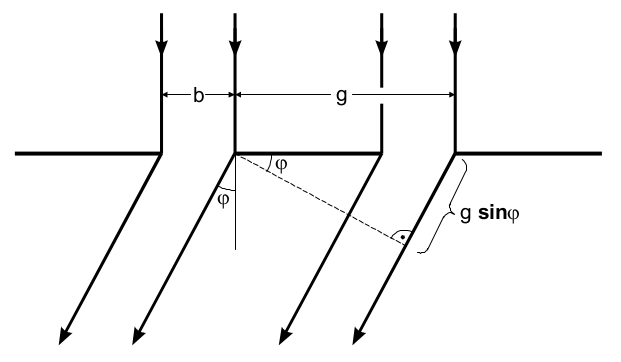
\includegraphics[height=5cm]{MeinFotoalbum:)/Spalt.png}
  \caption{Lichtbeugung an regelmäßig angeordneten Spaltöffnungen. $b$ ist die
  Spaltbreite und $g$ der Gangunterschied.\cite{anleitung}}
  \label{fig:Beugitter}
\end{figure}

\subsection{Ausmessung von Dublettlinien}
\label{sec:AvD}

Für den messbaren Abstand zwischen zwei Dublettlinien gilt gemäß Abbildung
\ref{fig:okular}
\begin{align}
  \increment s = r \increment \varphi.
  \label{eqn:okumess}
\end{align}
Mit Hilfe einer Eichmessung wird die Beziehung zwischen dem am Okularmikrometer
gemessenen Abstand und der Wellelänge aufgestellt
\begin{align}
  \increment t = r (\varphi_1 - \varphi_2).
  \label{eqn:eichung}
\end{align}
Mit einer Kleinwinkelnäherung ergibt sich für die Differenz der Wellenlängen
zwischen zwei Dublettlinien
\begin{align}
  \increment \lambda = g \cos(\bar{\varphi}) \increment \varphi,
\end{align}
wobei $\bar{\varphi}$ der gemittelte Wert zwischen beiden Dublettlinien ist.
Über die Beziehung \eqref{eqn:eichung} folgt dann
\begin{align}
  \increment \lambda = \frac{\cos \bar{\varphi}}{\cos \bar{\varphi}_{1,2}}
  \frac{\increment s}{\increment t} (\lambda_1 - \lambda_2).
\end{align}

\begin{figure}
  \centering
  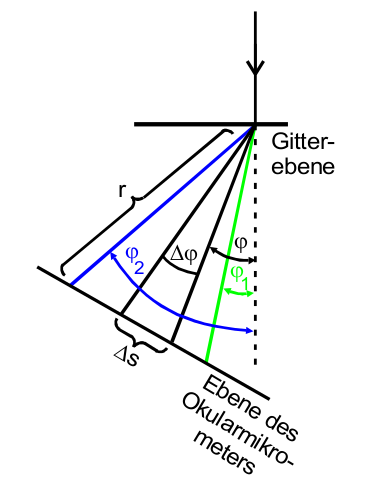
\includegraphics[height = 7cm]{MeinFotoalbum:)/DublettsMessung.png}
  \caption{Ausmessung der Dublettlinien mit Hilfe des Okularmikrometers.
  \cite{anleitung}}
  \label{fig:okular}
\end{figure}
